\hqlabel{subsubsection: Test-and-Test-and-Set lock}{\subsubsection{Test-and-Test-and-Set lock}}

The \definition{Test-and-Test-and-Set lock} mechanism improves upon the simple Test-and-Set lock by \textbf{reducing interconnect traffic and contention}. It \textbf{combines an initial test phase with a subsequent atomic Test-and-Set operation}.

\highspace
\begin{flushleft}
    \textcolor{Green3}{\faIcon{tools} \textbf{Implementation}}
\end{flushleft}
\begin{lstlisting}[language=C]
void Lock(int* lock) {
    while (1) {
        // Spin-wait until the lock appears free
        // (assume *lock is NOT register allocated)
        while (*lock != 0);

        // Try to acquire the lock atomically
        if (test_and_set(*lock) == 0)
            return;
    }
}

void Unlock(int* lock) {
    *lock = 0; // Release the lock
}    
\end{lstlisting}
\begin{itemize}
    \item \important{Initial Spin Phase}:
    \begin{itemize}
        \item \textbf{Purpose}: Processors continuously \textbf{check the value of the lock variable} (\texttt{*lock}) in a loop \textbf{until it becomes \texttt{0}} (free). This spin-wait phase helps reduce contention on the interconnect by delaying the atomic test-and-set operation until the lock appears free.
        \item \textbf{Implementation}: \texttt{while (*lock != 0);} causes the processor to repeatedly \textbf{check the lock value without sending any bus requests}.
    \end{itemize}
    
    \item \important{Atomic Test-and-Set Operation}:
    \begin{itemize}
        \item \textbf{Purpose}: Once the lock appears free, the \textbf{processor attempts to acquire it using the atomic \texttt{test\_and\_set} instruction}. This operation is performed in one \underline{uninterruptible step} to ensure that only one processor can acquire the lock at a time.
        \item \textbf{Implementation}: The line of code \texttt{if (test\_and\_set(*lock) == 0) return;} \textbf{checks if the lock was successfully acquired} (i.e., the function \texttt{test\_and\_set} returns \texttt{0}) \textbf{and exits the loop if it was}.
    \end{itemize}
    
    \item \important{Unlock Operation}:
    \begin{itemize}
        \item \textbf{Purpose}: To \textbf{release the lock}, the processor sets the lock variable back to \texttt{0}, indicating that the lock is free.
        \item \textbf{Implementation}: \texttt{*lock = 0;} simply sets the lock value to \texttt{0}.
    \end{itemize}
\end{itemize}

\newpage

\begin{flushleft}
    \textcolor{Red2}{\faIcon{exclamation-triangle} \textbf{Coherence Traffic}}
\end{flushleft}
\begin{figure}[!htp]
    \centering
    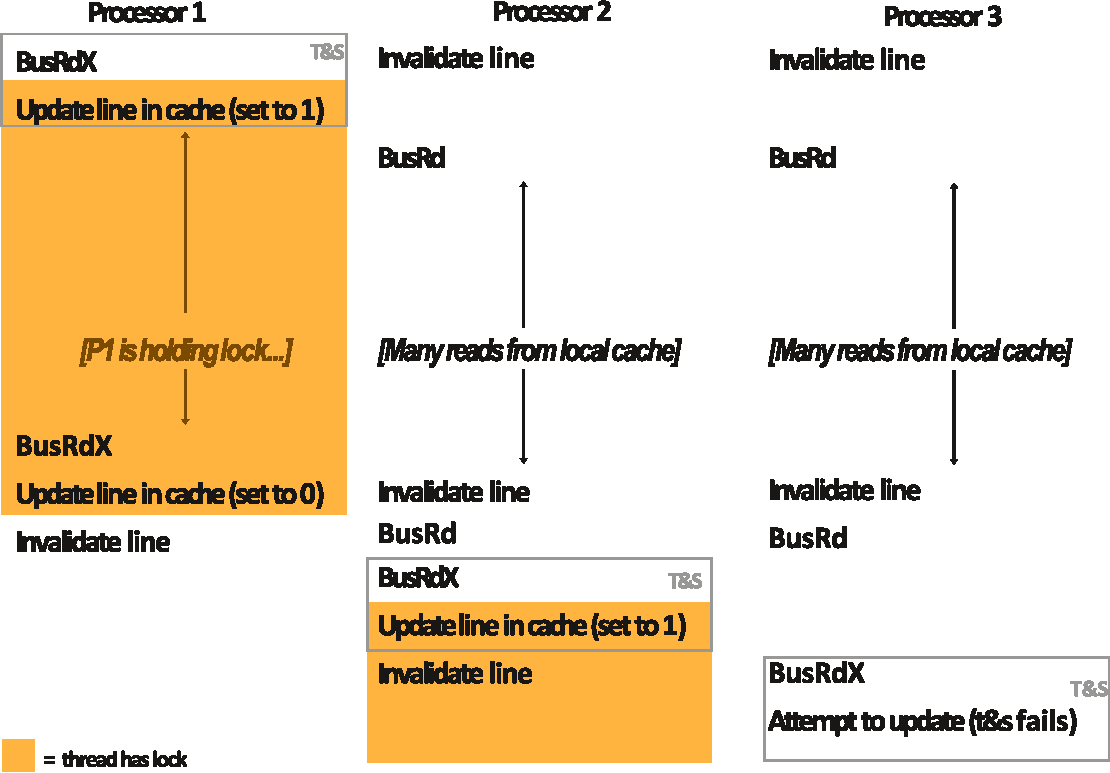
\includegraphics[width=\textwidth]{img/test-and-set-2.pdf}
\end{figure}
\begin{itemize}
    \item Processor 1 (\texttt{P1})
    \begin{itemize}
        \item \textbf{BusRdX}: \texttt{P1} sends a Bus Read Exclusive (\texttt{BusRdX}) request to acquire the lock.
        \item \textbf{Update Line in Cache}: \texttt{P1} updates its cache line, setting the lock value to \texttt{1}, indicating that it has acquired the lock.
        \item \textbf{[P1 is holding lock...]}: \texttt{P1} holds the lock and performs its critical section work.
        \item \textbf{BusRdX (Release)}: \texttt{P1} sends another BusRdX request when it releases the lock.
        \item \textbf{Update Line in Cache (Release)}: \texttt{P1} updates its cache line, setting the lock value to \texttt{0}, indicating that the lock is now free.
        \item \textbf{Invalidate Line}: Other processors' caches are invalidated for the lock variable.
    \end{itemize}

    \item Processor 2 (\texttt{P2})
    \begin{itemize}
        \item \textbf{Invalidate Line}: Initially, \texttt{P2}'s cache line for the lock is invalidated.
        \item \textbf{BusRd}: \texttt{P2} reads the lock value.
        \item \textbf{[Many Reads from Local Cache]}: \texttt{P2} spins, repeatedly reading the lock value from its local cache until it becomes free.
        \item \textbf{Invalidate Line}: When the lock is acquired/released, \texttt{P2}'s cache line is invalidated again.
        \item \textbf{BusRd}: \texttt{P2} reads the updated lock value.
    \end{itemize}

    \item Processor 3 (\texttt{P3})
    \begin{itemize}
        \item \textbf{Invalidate Line}: Initially, \texttt{P3}'s cache line for the lock is invalidated.
        \item \textbf{BusRd}: \texttt{P3} reads the lock value.
        \item \textbf{[Many Reads from Local Cache]}: \texttt{P3} spins, repeatedly reading the lock value from its local cache until it becomes free.
        \item \textbf{Invalidate Line}: When the lock is acquired/released, \texttt{P3}'s cache line is invalidated again.
        \item \textbf{BusRd}: \texttt{P3} reads the updated lock value.
        \item \textbf{BusRdX}: \texttt{P3} sends a \texttt{BusRdX} request to acquire the lock.
        \item \textbf{Update Line in Cache}: \texttt{P3} updates its cache line, setting the lock value to \texttt{1}, indicating that it has acquired the lock.
        \item \textbf{Invalidate Line}: Other processors' caches are invalidated for the lock variable.
        \item \textbf{BusRdX (Failed Attempt)}: If \texttt{P3}'s test-and-set operation fails (because another processor acquires the lock), it continues to spin and retry.
    \end{itemize}
\end{itemize}

\highspace
\begin{flushleft}
    \textcolor{Green3}{\faIcon{balance-scale} \textbf{Comparison with Test-and-Set}}
\end{flushleft}
\begin{itemize}
    \item \important{Slightly Higher Latency than Test-and-Set in Uncontended\break Cases}
    \begin{itemize}
        \item The test-and-test-and-set lock involves an \textbf{initial test phase} before the atomic test-and-set operation. This extra step \textbf{can introduce slightly higher latency when there is no contention}, as processors spend additional time in the spin-wait phase.
    \end{itemize}

    \item \important{Generates Much Less Interconnect Traffic}
    \begin{itemize}
        \item \textbf{One Invalidation per Waiting Processor per Lock Release}: Each waiting processor experiences one cache invalidation per lock release, resulting in $O(P)$ invalidations, where $P$ is the number of processors.
        \item \textbf{Comparison to Test-and-Set Lock}: The test-and-set lock generates one invalidation per waiting processor per test, leading to significantly higher interconnect traffic.
        \item $O(P^{2})$ \textbf{Interconnect Traffic}: If all processors have the lock cached, the interconnect traffic can be quadratic ($O\left(P^{2}\right)$). However, this is \textbf{still less than the traffic generated by the simple test-and-set lock}.
    \end{itemize}

    \item \important{More Scalable (Due to Less Traffic)}:
    \begin{itemize}
        \item \textbf{Scalability}: The reduced interconnect traffic makes the \textbf{test-and-test-and-set lock more scalable}. It can handle an increasing number of processors more efficiently than the simple test-and-set lock.
        \item \textbf{Impact}: As the number of processors grows, the performance impact of the test-and-test-and-set lock remains more manageable, making it suitable for larger multiprocessor systems.
    \end{itemize}

    \item \important{Storage Cost Unchanged (One Integer)}:
    \begin{itemize}
        \item \textbf{Storage Requirements}: The storage cost of the test-and-test-and-set lock remains the same as the simple test-and-set lock, requiring only one integer to represent the lock.
    \end{itemize}

    \item \important{Still No Provisions for Fairness}:
    \begin{itemize}
        \item \textbf{Fairness}\footnote{\definition{Fairness} in the context of lock mechanisms refers to the \textbf{equitable distribution of opportunities for multiple processors or threads to acquire the lock}. A fair locking mechanism ensures that all processors have a roughly equal chance of acquiring the lock, preventing any single processor from being starved of access to the critical section.}: The test-and-test-and-set lock does not include mechanisms to ensure fairness. This means that \textbf{some processors may experience longer waiting times to acquire the lock, leading to potential starvation}.
        \item \textbf{Implications}: While the lock reduces interconnect traffic and improves scalability, the lack of fairness can still be a significant drawback in systems where equitable access to resources is important.
    \end{itemize}
\end{itemize}
The \textbf{test-and-test-and-set locking mechanism offers several advantages} over the simple test-and-set lock, including \example{reduced interconnect traffic} and \example{improved scalability}. However, it introduces \important{slightly higher latency in uncontended cases} and \important{does not address fairness issues}. Overall, it is a more efficient and scalable locking solution for multiprocessor systems, though not without its limitations.
